\documentclass[12pt, twoside]{article}
\usepackage[letterpaper, margin=1in, headsep=0.5in]{geometry}
\usepackage[english]{babel}
\usepackage[utf8]{inputenc}
\usepackage{amsmath}
\usepackage{amsfonts}
\usepackage{amssymb}
\usepackage{tikz}
\usepackage{yhmath}
%\usetikzlibrary{quotes, angles}

\usepackage{graphicx}
\usepackage{enumitem}
\usepackage{multicol}

\usepackage{fancyhdr}
\pagestyle{fancy}
\fancyhf{}
\renewcommand{\headrulewidth}{0pt} % disable the underline of the header

\fancyhead[RE]{\thepage}
\fancyhead[RO]{\thepage \\ Name: \hspace{3cm}}
\fancyhead[L]{BECA / Dr. Huson / 10th Grade Geometry\\* 10 May 2019}

\begin{document}
\subsubsection*{10.12 Unit Exam: Volume, density, trigonometry, \& review}
 \begin{enumerate}

  \item Find the area of a semi-circle with diameter 8. Round to the \emph{nearest tenth}.\vspace{3cm}

  \item Find the volume of a cylindrical tank with radius of $6$ feet and a height of 8 feet, to the \emph{nearest cubic foot}. \vspace{2.5cm}

  \item A box in the shape of a rectangular prism has a volume of 60 cubic feet. It's length is 5 feet and width 3 feet. How tall is it? \vspace{3.0cm}

  \item The area of $\triangle ABC$ is $68.25$ square inches. The altitude of the triangle is $6.5$ inches. Find the length of the base $AB$.\\[0.5cm]
  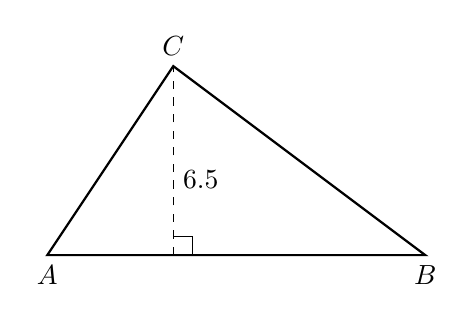
\begin{tikzpicture}[scale=0.8]
   \draw [thick]
     (0,0)node[below]{$A$}--
     (6,0)node[below]{$B$}--
     (2,3)node[above]{$C$} --cycle;
  \draw [dashed] (2,0)--(2,3);
  \draw (2,0)++(0.3,0)--++(0,0.3)--+(-0.3,0);
  \node at (2,1.2)[right]{$6.5$};
  %\node at (3,0)[below]{$20.7$};
\end{tikzpicture} \vspace{0.25cm}

  \item Find the weight of a steel ball with a diameter of 1.4 inches, to the \emph{nearest tenth of an ounce}. (The density of steel is 4.6 ounce per cubic inch)

\newpage

  \item A circle with a diameter of 12 in and a central angle of $80^\circ$ is drawn below. What is the area of the sector formed by the $80^\circ$ angle, to the \emph{nearest tenth of a square inch}?\\[0.25cm]
       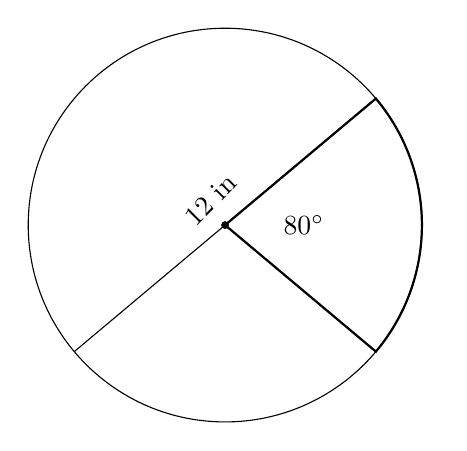
\begin{tikzpicture}[scale=.5]
         \draw (0,0) circle[radius=5];
         \draw (40:5)--(220:5);
         %\draw (0,0)--(-40:5);
         \fill (0,0) circle[radius=0.1];
         \draw (0:2) node{$80^\circ$};
         \draw (120:0.75) node[rotate=45]{$12$ in};
         \draw [thick] (0,0)--(-40:5) arc [start angle=-40, end angle=40, radius=5]
         --cycle;
       \end{tikzpicture}
   \vspace{0.5cm}

  \item A bakery sells hollow chocolate spheres. The outer diameter of each sphere is 6 cm. The thickness of the chocolate of each sphere is 1 cm. Determine and state, to the \emph{nearest tenth of a cubic centimeter}, the amount of chocolate in each hollow sphere.\\[0.5cm]
  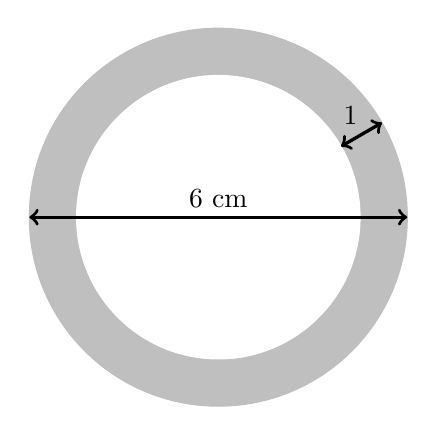
\begin{tikzpicture}[scale=1.2]
    \draw [fill, color=lightgray] (0,0) circle[radius=2];
    \draw [fill, color=white] (0,0) circle[radius=1.5];
    \draw [very thick, <->] (0:2)--(180:2);
    \draw (0,0) node[above]{$6$ cm};
    \draw [very thick, <->]  (30:1.5)--(30:2);
    \draw (32:1.65) node[above]{$1$};
  \end{tikzpicture} \vspace{1.25cm}

  \item A right cylinder is cut horizontally. The shape of the cross section is a
    \begin{enumerate}
      \item circle
      \item cylinder
      \item rectangle
      \item triangular prism
    \end{enumerate}

  \item Which three-dimensional figure will result when a right triangle 8 inches tall and 3 inches wide is continuously rotated about the longer side?
    \begin{enumerate}
      \item a cone with a height of 6 inches and radius of 8 inches
      \item a cone with a height of 8 inches and diameter of 6 inches
      \item a cylinder with a radius of 8 inches and a height of 6 inches
      \item a cylinder with a diameter of 6 inches and a height of 8 inches
    \end{enumerate}

\newpage

  \item $\triangle ABC$ is shown with $m\angle C=90^\circ$ and the lengths of the triangle's sides are $BC=3$, $AC=4$, and $AB=5$.
  \begin{multicols}{2}
        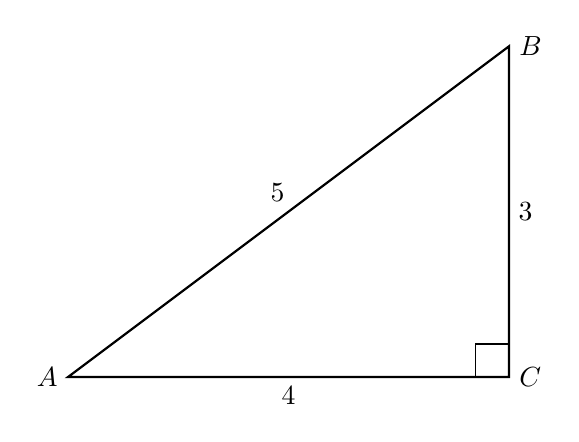
\begin{tikzpicture}[scale=0.7]
          \draw [thick]
          (0,0)node[left]{$A$}--
          (8,0)node[ right]{$C$}--
          (8,6)node[right]{$B$}--cycle;
          \draw (8,0)++(-0.6,0)--++(0,0.6)--+(0.6,0);
          \node at (4,0)[below]{$4$};
          \node at (8,3)[right]{$3$};
          \node at (3.8,3)[above]{$5$};
        \end{tikzpicture}
        \begin{enumerate}
        \item State, as a decimal, the value of $\sin A$. \vspace{1.25cm}
        \item Find the measure of $\angle A$, to the \emph{nearest degree}. \vspace{1.25cm}
        \item Find the degree measure of $\angle B$.
      \end{enumerate}
    \end{multicols}
    \vspace{1.5cm}

  \item Express each trigonometric ratio to the \emph{nearest thousandth} and each angle measure to the nearest degree.
    \begin{multicols}{2}
      \begin{enumerate}
        \item $\sin 55^\circ =$ \vspace{0.5cm}
        \item $\cos^{-1} 0.766 =$ \vspace{0.5cm}
      \end{enumerate}
    \end{multicols} \vspace{0.25cm}

  \item A sailor observes the top of a lighthouse with an angle of elevation of $5^\circ$. She knows the lighthouse is 90 feet tall. Determine and state the distance $x$ between the sailor and the lighthouse, to the \emph{nearest foot}.\\[0.5cm]
    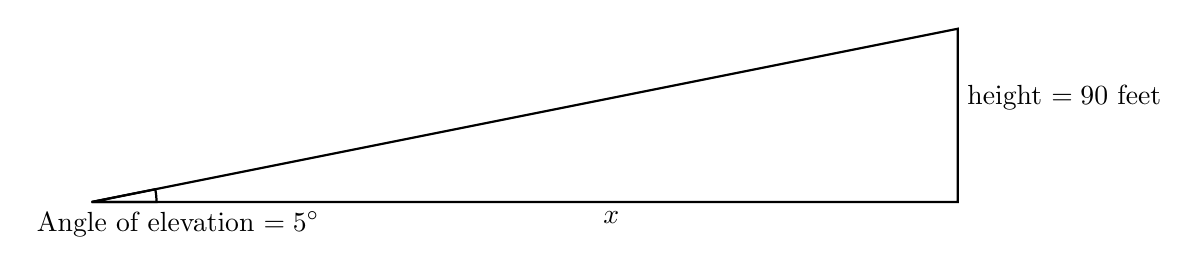
\begin{tikzpicture}[scale=1.1]
     \draw [thick] (10,0)--(0,0)--(10,2.0)--cycle;
     \draw [thick] (0,0)--(0.75,0) arc [start angle=0, end angle=11.3, radius=0.75]--cycle;
     \node at (1,0)[below]{Angle of elevation $=5^\circ$};
     \node at (10,1.2)[right]{height $=90$ feet};
     \node at (6,0)[below]{$x$};
    \end{tikzpicture} \vspace{3.25cm}

\newpage
  \item   Solve for the value of $x$.\\[0.5cm]
  $\frac{1}{3}(4x+1)=3$ \vspace{3cm}

  \item Given $f(x)=\frac{3}{2} x-5$. Solve for $x$ such that for $f(x)=1$. \vspace{3.5cm}
  \item Given $g(x)=2x^2-3x+2$. Simplify $g(0)$. \vspace{4cm}
  \item Given $h(x)=x^2+8x+7$. Solve $h(x)=0$. \vspace{5cm}

  \item Simplify each expression. (Leave it in radical form if necessary, not a decimal.)
    \begin{enumerate}
      \begin{multicols}{2}
      \item   $\sqrt{18}$ \vspace{1.25cm}
      \item   $\sqrt{\frac{81}{16}}$ \vspace{1.25cm}
      \end{multicols}
    \end{enumerate}


\newpage
  \item The line $l$ has the equation $y=\frac{2}{3}x+7$. To each line below, circle whether $l$ is parallel, perpendicular, or neither.
    \begin{enumerate}
      \item parallel \quad perpendicular \quad neither \qquad $y=\frac{2}{3}x-2$
      \vspace{0.5cm}
      \item parallel \quad perpendicular \quad neither \qquad $y=\frac{3}{2}x+7$
      \vspace{0.5cm}
      \item parallel \quad perpendicular \quad neither \qquad $y=-\frac{2}{3}x+5$
      \vspace{0.5cm}
      \item parallel \quad perpendicular \quad neither \qquad $3x+2y=6$
      \vspace{3.5cm}
    \end{enumerate}

  \item Write an equation of the line that is parallel to the line whose equation is $y=\frac{1}{3}x+4$ and passes through the point $(4,-1)$. \vspace{2cm}

  \item Given $m\angle R=30$ and $m\angle U=70$. Find $m\angle UST$.\\[1cm]
  \begin{tikzpicture}
   %\draw [->, thick] (0,0)--(5,5);
   \draw [<-, thick] (8,0)--(0,0)--(3,3)--(4.5,0);
   \draw [fill] (0,0) circle [radius=0.05] node[below]{$R$};
   \draw [fill] (4.5,0) circle [radius=0.05] node[below]{$S$};
   \draw [fill] (3,3) circle [radius=0.05] node[right]{$U$};
   \draw [fill] (7,0) circle [radius=0.05] node[below]{$T$};
  \end{tikzpicture} \vspace{1cm}

  \item Write down the center and radius of each circle.
   \begin{enumerate}
     \begin{multicols}{2}
     \item   $(x+1)^2+(y+3)^2=1$ \vspace{2.5cm}
     \item   $x^2+(y-4)^2=25$ \vspace{2.5cm}
     \end{multicols}
   \end{enumerate} \vspace{2cm}

  \newpage
  \item In the diagram below, $\overline{AC}$ has endpoints with coordinates $A(-3,1)$ and $C(6,4)$.
   \begin{center} %4 quadrant regents grid
     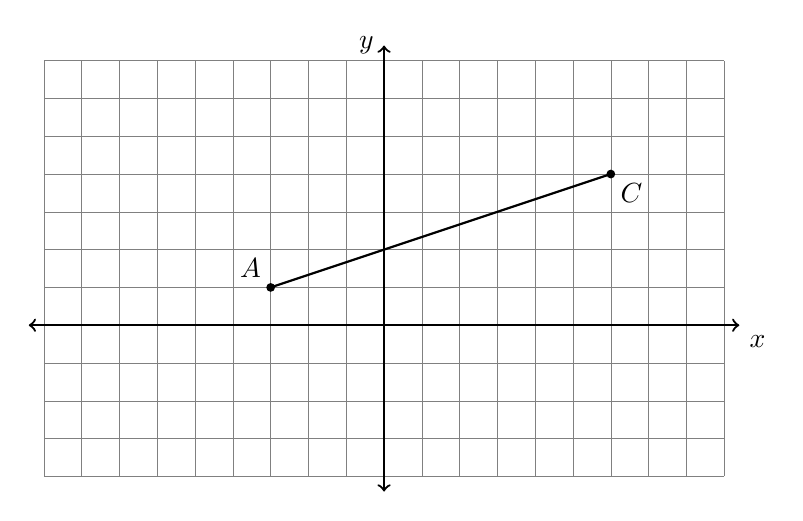
\begin{tikzpicture}[scale=.48]
       \draw [help lines] (-9,-4) grid (9,7);
       \draw [thick, <->] (-9.4,0) -- (9.4,0) node [below right] {$x$};
       \draw [thick, <->] (0,-4.4)--(0,7.4) node [left] {$y$};
       \draw [thick] (-3, 1)--(6,4);
       \draw [fill] (-3, 1) circle [radius=0.1] node[above left] {$A$};
       \draw [fill] (6, 4) circle [radius=0.1] node[below right] {$C$};
     \end{tikzpicture}
   \end{center}
   If $B$ is a point on $\overline{AC}$ and $AB {:} BC = 2{:}1$,  what  are  the coordinates of $B$? \vspace{4cm}

  \item Triangle $ABC$ is dilated with a scale factor of $k$ centered at $A$, yielding $\triangle ADE$, as shown. Given $AB=8$, $BC=10$, $AC=12$, and $DE=15$. \\[0.25cm] Find $BD$, $AE$, and $k$ (the scale factor).\\[0.25cm]
     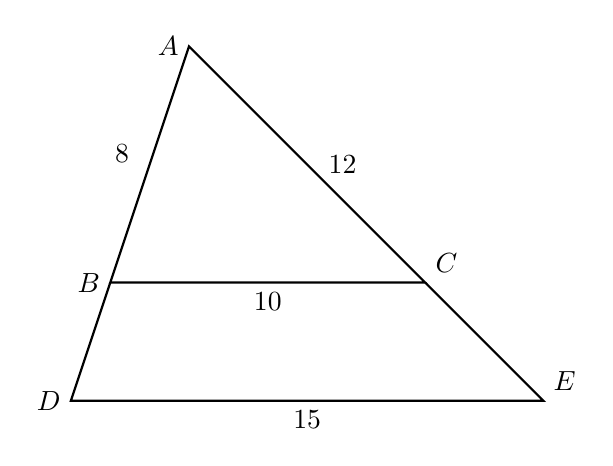
\begin{tikzpicture}[scale=0.5]
       \draw [thick]
       (0,0)node[left]{$B$}--
       (8,0)node[above right]{$C$}--
       (2,6)node[left]{$A$}--cycle;
       \draw [thick]
       (0,0)--
       (-1,-3)node[left]{$D$}--
       (11,-3)node[above right]{$E$}--(8,0);
       \node at (4,0)[below]{$10$};
       \node at (5.3, 3)[right]{$12$};
       \node at (0.3, 2.8)[above]{$8$};
       \node at (5,-3)[below]{$15$};
     \end{tikzpicture}
  \vspace{2cm}

\newpage
  \item What is the smallest non-zero angle of rotation about its center that would map the pentagon onto itself? \vspace{0.25cm}
  \begin{center}
    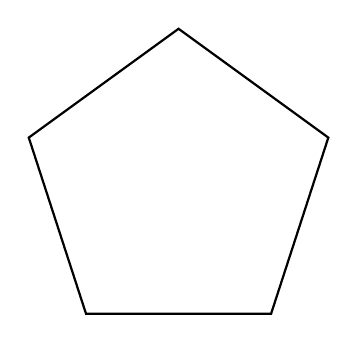
\begin{tikzpicture}%[scale=.48]
      \draw [thick]
      (18:2)--
      (90:2)--
      (162:2)--
      (234:2)--
      (306:2)--cycle;
    \end{tikzpicture}
  \end{center} \vspace{1cm}

  \item A translation maps $A(-1,4) \rightarrow A'(-2,14)$. What is the image of $B(-4,-7)$ under the same translation?  \vspace{2.5cm}

  \item What transformation maps $\triangle ABC$ onto $\triangle DEF$, shown below? Fully specify the transformation.
    \begin{center}
      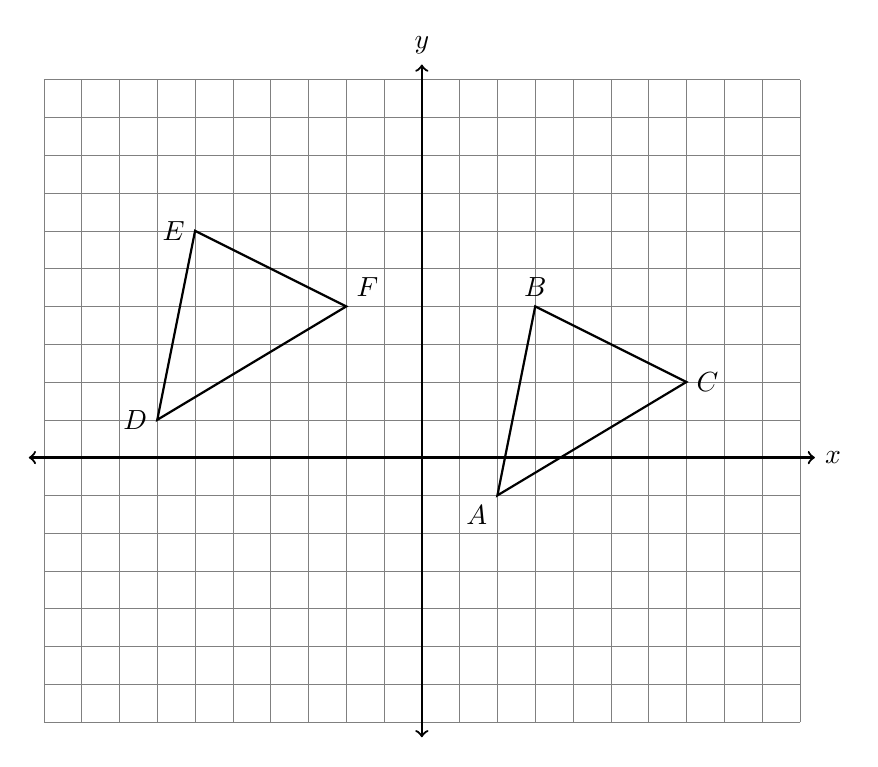
\begin{tikzpicture}[scale=.48]
        \draw [help lines] (-10,-7) grid (10,10);
        \draw [thick, <->] (-10.4,0) -- (10.4,0) node [right] {$x$};
        \draw [thick, <->] (0,-7.4)--(0,10.4) node [above] {$y$};
        \draw [thick]
          (2,-1) node[below left] {$A$}--
          (3,4) node[above] {$B$}--
          (7,2) node[right] {$C$}--cycle;
        \draw [thick]
          (-7,1) node[left] {$D$}--
          (-6,6) node[left] {$E$}--
          (-2,4) node[above right] {$F$}--cycle;
      \end{tikzpicture}
    \end{center}

\newpage
  \item Reflect $\triangle PQR$ across the $x$-axis, drawing its image $\triangle P'Q'R'$ and labeling its vertices.
    \begin{center}
      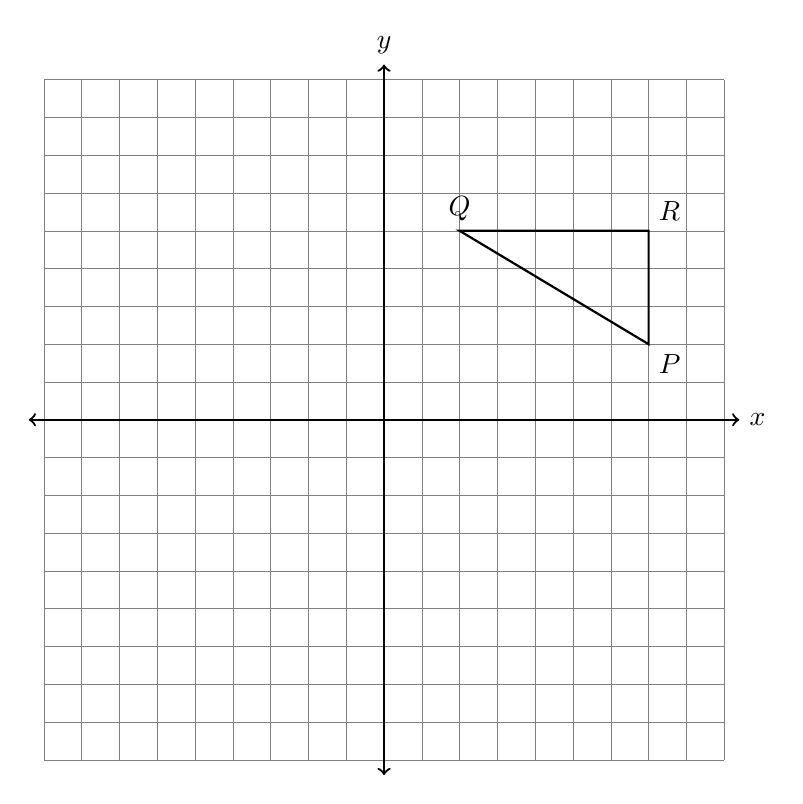
\begin{tikzpicture}[scale=.48]
        \draw [help lines] (-9,-9) grid (9,9);
        \draw [thick, <->] (-9.4,0) -- (9.4,0) node [right] {$x$};
        \draw [thick, <->] (0,-9.4)--(0,9.4) node [above] {$y$};
        \draw [thick]
          (7,2) node[below right] {$P$}--
          (2,5) node[above] {$Q$}--
          (7,5) node[above right] {$R$}--cycle;
      \end{tikzpicture}
    \end{center}

  \item In a right triangle, the acute angles have the relationship $\sin x=\cos 30$. Find x. \vspace{2.0cm}

  \item If $\sin (2x-8)^\circ = \cos 42^\circ$, what is the value of $x$? \vspace{3cm}

  \item Find the distance between $(0,5)$ and $(6, -3)$. \vspace{3cm}

\newpage
  \item Given circle $O$ with inscribed $\triangle AOB$. $m\angle O=110$. Find $m\angle A$.\\[1cm]
      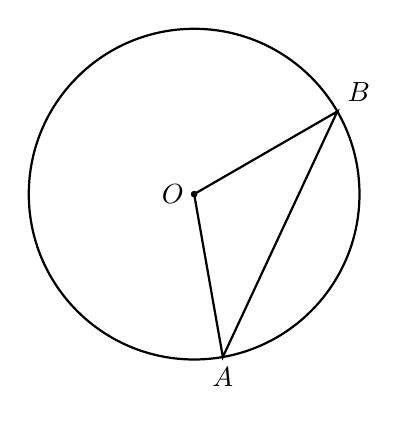
\begin{tikzpicture}[scale=0.7]
        %\draw [-, thick] (-6,0) node[left]{$A$}--(0,0);
        \draw  [thick] (0,0) circle [radius=3] node[left]{$O$};
        \draw [thick] (-80:3) node[below]{$A$}--(0,0)
          --(30:3) node[above right]{$B$}--cycle;
        \draw [fill] (0,0) circle [radius=0.05];
      \end{tikzpicture} \vspace{1cm}

  \item Given circle $P$ with $m \angle APB=74^\circ$.
    \begin{multicols}{2}
     \raggedcolumns
     \begin{enumerate}
       \item Write down the $m \wideparen{AB}$. \vspace{1.7cm}
       \item Find the $m\angle AQB$. \vspace{2cm}
     \end{enumerate}
       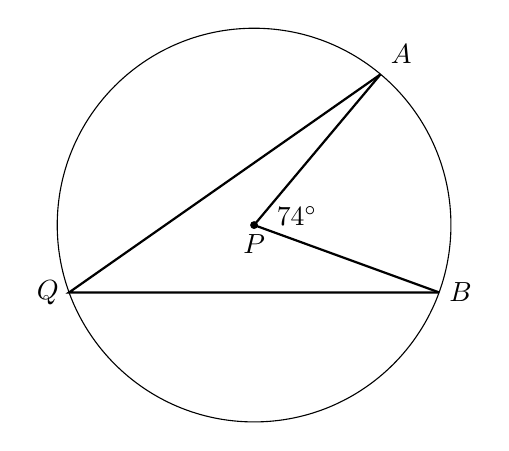
\begin{tikzpicture}[scale=.5]
         \draw (0,0) circle[radius=5];
         \draw [thick]
         (-20:5) node[right] {$B$}--
         (0,0) --
         (50:5) node[above right] {$A$};
         \draw [thick] (-20:5)--(200:5) node[left] {$Q$}--(50:5);
         \draw (35:0.4) node[right]{$74^\circ$};
         \fill (0,0) circle[radius=0.1] node[below]{$P$};
       \end{tikzpicture}
    \end{multicols}

  \item The secants $\overline{ABC}$ and $\overline{ADE}$ intersect the circle $O$, as shown in the diagram. \\Given $m \wideparen{BD}=40^\circ$ and $m \wideparen{CE}=160^\circ$. Find the $m\angle A$.
   \begin{center}
   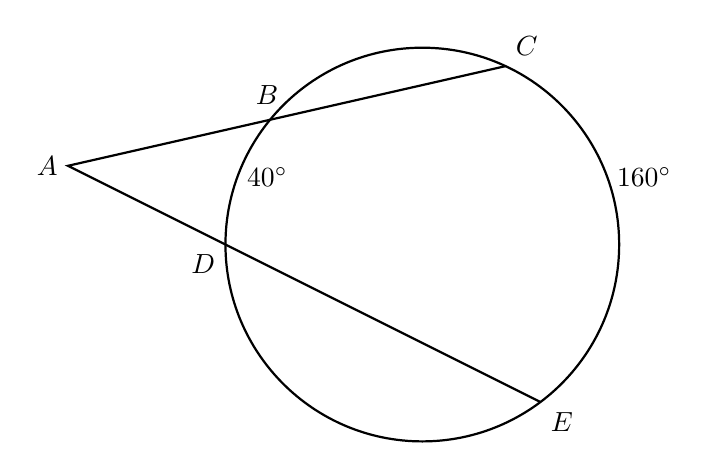
\begin{tikzpicture}[scale=.5]
     \draw [thick] (0,0) circle[radius=5];
     \draw [thick]
     (3,-4) node[below right] {$E$}--
     (-5,0) node[below left] {$D$}--
     (-9,2) node[left] {$A$}--
     (65:5) node[above right] {$C$};
     \draw (132:5.1) node[left] {$B$};
     \draw (20:5) node[right] {$160^\circ$};
     \draw (160:5) node[right] {$40^\circ$};
   \end{tikzpicture}
 \end{center} \vspace{2cm}

\newpage

  \item On the set of axes below, $\triangle ABC$, altitude $\overline{GC}$, and  median $\overline{MC}$ are drawn.
    \begin{center}
      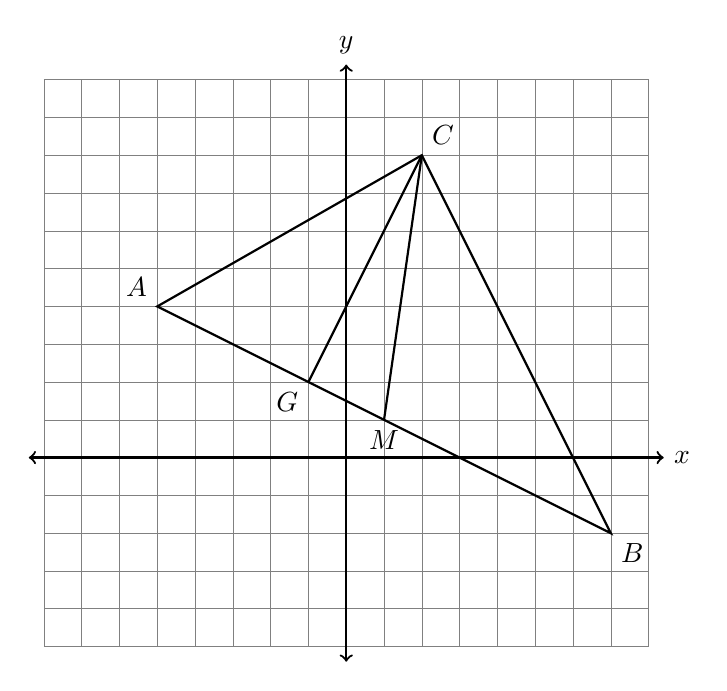
\begin{tikzpicture}[scale=.48]
        \draw [help lines] (-8,-5) grid (8,10);
        \draw [thick, <->] (-8.4,0) -- (8.4,0) node [right] {$x$};
        \draw [thick, <->] (0,-5.4)--(0,10.4) node [above] {$y$};
        \draw [thick]
          (-5,4) node[above left] {$A$}--
          (7,-2) node[below right] {$B$}--
          (2,8) node[above right] {$C$}--
          cycle;
        \draw [thick] (1,1) node[below] {$M$}--(2,8);
        \draw [thick] (-1,2) node[below left] {$G$}--(2,8);
      \end{tikzpicture}
    \end{center}
      Determine which equations represent the area of the triangle, circling True or False.
      \begin{multicols}{2}
       \begin{enumerate}
          \item \quad T \quad F \quad $\displaystyle Area_\triangle = \frac{(CG)(AB)}{2}$
          \item \quad T \quad F \quad $\displaystyle Area_\triangle = \frac{(CM)(AB)}{2}$ \vspace{0.25cm}
          \item \quad T \quad F \quad $\displaystyle Area_\triangle = \frac{(AC)(AB)}{2}$ \vspace{0.25cm}
          \item \quad T \quad F \quad $\displaystyle Area_\triangle = \frac{(CG)(BC)}{2}$
      \end{enumerate}
      \end{multicols}
      \vspace{0.25cm}

  \item The point $M(3,7)$ is the midpoint of $\overline{AB}$. If the coordinates of $A$ are $(2,10)$, find $B$. \vspace{2.5cm}

  \item A monument in the shape of a pyramid with a square base has a volume of 128 cubic feet. If its height measures 6 feet, what is the length of the side of the base? \vspace{3.5cm}

\newpage
\subsubsection*{Early finishers}

  \item A staircase riser is cut as a series of congruent triangles with each step's ``rise" equal to 6.75 inches, and the ``run" of each step is 8.25 inches, as shown below. ($AB=6.75$ and $BC=8.25$)
  \begin{enumerate}
    \item What is the angle of inclination of the staircase, $x$, rounded to the \emph{nearest degree}?\\[0.5cm] 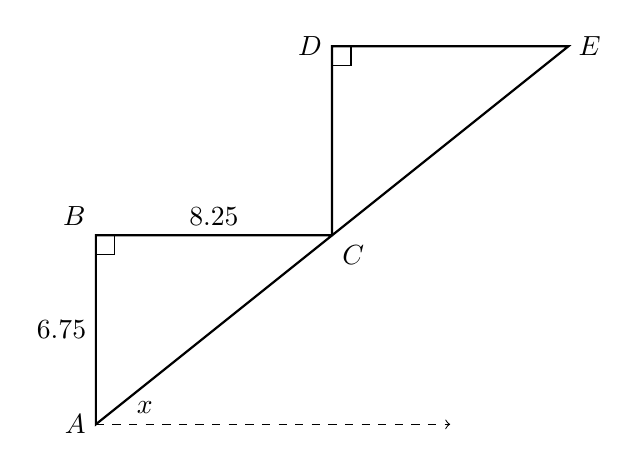
\begin{tikzpicture}[scale=0.3]
          \draw [thick]
          (0,0)node[left]{$A$}--
          (0,8)node[above left]{$B$}--
          (10,8)node[below right]{$C$}--
          (10,16)node[left]{$D$}--
          (20,16)node[right]{$E$}--cycle;
          \draw [dashed, ->] (0,0)--(15,0);
          \draw (0,8)++(0,-0.8)--++(0.8,0)--+(0,0.8);
          \draw (10,16)++(0,-0.8)--++(0.8,0)--+(0,0.8);
          \node at (0,4)[left]{$6.75$};
          \node at (5,8)[above]{$8.25$};
          \node at (28:1.5)[right]{$x$};
        \end{tikzpicture}
      \item Find the diagonal length of the two-step riser, the distance $AE$, to the \emph{nearest tenth of an inch}.
    \end{enumerate} \vspace{2.5cm}

  \item Given circle $O$ with chords $\overline{AD}$ and $\overline{BE}$ intersecting at $C$, as shown in the diagram. Given $m \wideparen{AB}=86^\circ$, $m \wideparen{BD}=75^\circ$, and $m \wideparen{DE}=50^\circ$.
    \begin{multicols}{2}
     \raggedcolumns
     \begin{enumerate}
       \item Find the $m\angle ACB$. \vspace{3.5cm}
       \item Find the measure of the minor arc, $m\wideparen{AE}$. \vspace{2cm}
     \end{enumerate}
     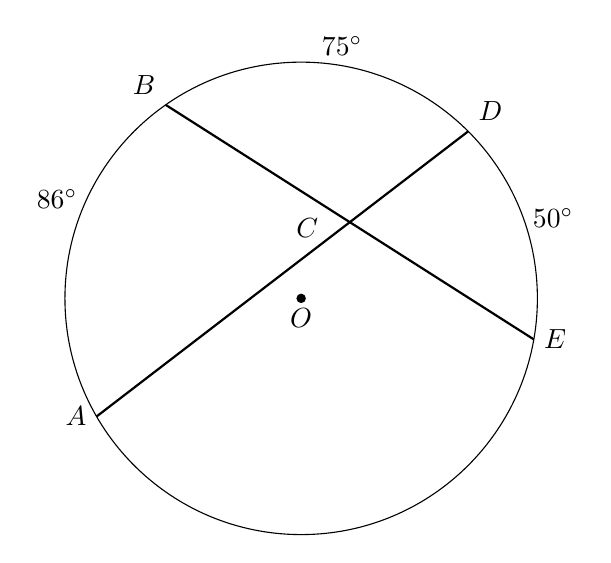
\begin{tikzpicture}[scale=.6]
       \draw (0,0) circle[radius=5];
       \draw [thick]
       (-10:5) node[right] {$E$}--
       (125:5) node[above left] {$B$};
       \draw [thick] (210:5) node[left] {$A$}--
       (45:5) node[above right] {$D$};
       \draw (85:1.5) node{$C$};
       \draw (20:5) node[right] {$50^\circ$};
       \draw (80:5) node[above] {$75^\circ$};
       \draw (155:5) node[left] {$86^\circ$};
      \fill (0,0) circle[radius=0.1] node[below]{$O$};
     \end{tikzpicture}
    \end{multicols}  \vspace{2cm}


\end{enumerate}
\end{document}


        \item The map of a campground is shown below. Campsite C, first aid station F, and supply station S lie along a straight path. The path from the supply station to the tower, T, is perpendicular to the path from the supply station to the campsite. The length of path FS is 400 feet. The angle formed by path TF and path FS is $72^\circ$. The angle formed by path   and path CS is $55^\circ$.\\[0.5cm]
        \includegraphics[width=0.5\textwidth]{camp_Jun2018-31.png}
          \begin{enumerate}
            \item Determine and state the volume of concrete needed, \emph{in cubic feet}. \vspace{1cm}
            \item Sarah can mix her own concrete for \$3.25 per cubic foot. How much money will it cost her to replace the two concrete sections?
        \end{enumerate} \vspace{2.5cm}
